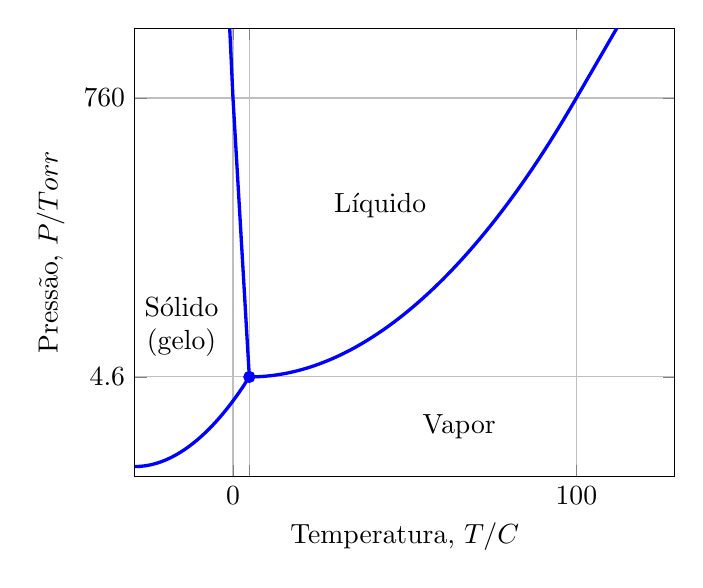
\begin{tikzpicture}
\begin{axis}
    [
        grid = major,
        ylabel = {Pressão, $P/\unit{Torr}$},
        xlabel = {Temperatura, $T/\unit{\degree C}$},
        ymin=0, ymax=900,
        xmin=-35, xmax=130,
        xtick = {-5, 0, 100},
        xticklabels = {0, , 100},
        ytick = {200, 760},
        yticklabels = {4.6, 760},
    ]       
    \draw [draw=blue, very thick]
        (axis cs: -35, 20) parabola 
        (axis cs: 0, 200);
    \draw [draw=blue, very thick]
        (axis cs: 0, 200) --
        (axis cs: -5, 760) --
        (axis cs: -6, 900);
    \draw [draw=blue, very thick]
        (axis cs: 0, 200) parabola
        (axis cs: 100, 760) --
        (axis cs: 130, 1100);

    \addplot [ mark=*, color=blue, only marks ] coordinates
        { 
            (0, 200)
        };

    \node [anchor = west, align = center] at (axis cs:-35, 300) 
        { Sólido \\ (gelo) };
    \node [anchor = south] at (axis cs:40, 500) 
        { Líquido };
    \node [anchor = west] at (axis cs:50, 100) 
        { Vapor };
\end{axis}
\end{tikzpicture}
